\documentclass[t]{beamer}
\usepackage[danish]{babel}
 \usepackage[utf8]{inputenc} % til at skrive æÆøØåÅ.
\usepackage{amsmath,amssymb,amsfonts,amsthm,mathrsfs,latexsym}
\usepackage{tikz}
\usepackage{diagbox} % til at lave diagonal i tabelcelle
\usepackage{graphicx}% til at rette størrelsen af tabel
\usepackage{mathtools}
\usepackage[normalem]{ulem} % strikethrough on text: command \sout{text}

% Beamer setup
\usetheme[nat]{Frederiksberg}


% Titlepage
\title{En Introduktion til Gruppeteori}
\subtitle{}

\author{Rasmus Juhl Christensen og Nicolai Sebastian Carstensen}
\institute{stud.scient \\ Københavns Universitet}
\date{21. september 2019}

% Commands
\newcommand{\cupdot}{\mathbin{\mathaccent\cdot\cup}}

\newcommand{\mN}{\mathbb{N}}
\newcommand{\mZ}{\mathbb{Z}}
\newcommand{\mQ}{\mathbb{Q}}
\newcommand{\mR}{\mathbb{R}}
\newcommand{\mC}{\mathbb{C}}
\newcommand{\mP}{\mathbb{P}}
\newcommand{\mA}{\mathbb{A}}

\newcommand{\mH}{\mathbb{H}}
\newcommand{\mD}{\mathbb{D}}

\newcommand{\cM}{\mathcal{M}}
\newcommand{\cH}{\mathcal{H}}
\newcommand{\cD}{\mathcal{D}}
\newcommand{\cF}{\mathcal{F}}
\newcommand{\cC}{\mathcal{C}}
\newcommand{\cSH}{\mathcal{SH}}

\newcommand{\M}{\text{M}}
\newcommand{\SL}{\text{SL}}
\newcommand{\GL}{\text{GL}}
\newcommand{\SO}{\text{SO}}
\newcommand{\PSL}{\text{PSL}}
\renewcommand{\d}{\hspace{1mm}d}


\newcommand{\floor}[1]{\left\lfloor #1\right\rfloor}
\newcommand{\ceil}[1]{\left\lceil #1\right\rceil}
\newcommand{\leg}[2]{\left(\frac{#1}{#2}\right)}

\newcommand{\ths}{\hspace{0.5mm}}
\newcommand{\hs}{\hspace{1mm}}
\newcommand{\Hs}{\hspace{4mm}}
\newcommand{\HS}{\hspace{8mm}}

\newcommand{\abs}[1]{\left| #1\right|}
\newcommand{\pare}[1]{\left( #1\right)}
\newcommand{\bigPare}[1]{\bigg( #1\bigg)}
\newcommand{\cbrac}[1]{\left\{ #1\right\}}
\newcommand{\setBrac}[2]{\left\{ #1 \hs\middle|\hs #2 \right\}}
\newcommand{\brac}[1]{\left[ #1\right]}
\newcommand{\norm}[1]{\left\lVert#1\right\rVert}
\newcommand{\inProd}[1]{\left\langle#1\right\rangle}

\renewcommand{\Im}{\text{Im}\hs}
\renewcommand{\Re}{\text{Re}\hs}
\renewcommand{\phi}{\varphi}
\newcommand{\ord}{\text{ord}}
\newcommand{\supp}{\text{supp}\hs}
\newcommand{\Aut}[1]{\text{Aut}(#1)}
\newcommand{\stab}[2]{\text{Stab}_{#1}\pare{#2}}
\newcommand{\cusp}[1]{\text{Cusps}\pare{#1}}
\newcommand{\dist}[1]{\text{dist}\pare{#1}}

\newcommand{\nl}{\newline \\}

\begin{document}

\begin{frame}
	\maketitle
\end{frame}

\section{Introduktion}

\begin{frame}{Introduktion}
\onslide<1->{
Vi skal denne weekend arbejde med at tilgå stof:
}

\onslide<2->{
\textbf{Undersøgende}. \\

Vi arbejder med konkrete eksempler og leder efter mønstre og strukturer. \nl
}


\onslide<3->{
\textbf{Abstraherende}.\\
Vi arbejder med at kunne begå os i rent abstrakte strukturer.
\nl
}


\onslide<4->{
\textbf{Udfordrende}. \\
Vi arbejde med at udfordre de fremkomne aksiomer og definitioner. \nl
}

\onslide<5->{
\textbf{Konkretiserende}.\\
Vi arbejder med at konkretisere abstrakte resultaters anvendelse.
}
\end{frame}

\begin{frame}{Repetition af modulær aritmetik}
\onslide<1->{
\textbf{Definition}. \\
Lad $n\in \mN$, og betragt relationen $\equiv$ på $\mZ$ givet ved
$$a\equiv b \Leftrightarrow n \mid a-b.$$
Hvis $a\equiv b$ siger vi, at $a$ er kongruent med $b$ modulo $n$. \nl
}


\onslide<2->{
\textbf{Definition}. \\
Lad $n\in \mZ$ og lad $a,b\in \mZ$. Vi definerer addition og multiplikation i $\mZ/n\mZ$ på følgende måde:
\begin{itemize}
\item $[a]+[b]=[a+b]$
\item $[a][b]=[ab]$
\end{itemize}
}

\onslide<3->{
\textit{Spørgsmål}:
Er disse veldefineret?
}

\end{frame}


\begin{frame}{Matematiske strukturer}
\onslide<1->{
\textbf{Motivation}. \\
Vi ønsker nu at motivere vores arbejde denne weekend med en \textit{undersøgende} tilgang til nogle konkrete eksempler.  \nl
}


\onslide<2->{
\textbf{Mål}. \\
I denne øvelse tiltænkes I at:
\begin{itemize}
\item<3-> Opdage mønstre i konkrete eksempler
\item<4-> Udfordre disse mønstre i lignende opstillede eksempler
\item<5-> Finde fællestræk og forskelle på tværs af eksempler
\item<6-> Introducere en fælles terminologi til karakterisering af eksempler
\end{itemize}
}
\end{frame}
\begin{frame}{Motivation for Abstrakt Algebra}
\onslide<1->{
\textbf{Opsamling}.\\
Vi har arbejdet med:
\begin{itemize}
\item Mængder,
\item operationer
\item og samspillet mellem de to
\end{itemize}
}
\onslide<2->{
\vspace{3mm}
\textbf{Mængder}.
\begin{itemize}
\item<3-> Vi har talt om talmængder, herunder $\mN,\hs\mZ,\hs\mQ,\hs\mR$ og $\mC$.
\item<4-> Vi har talt om mængden af restklasser, herunder $\mZ/n\mZ$
\item<5-> Vi har talt om mængden af rotationer og spejlinger \\
\end{itemize}
}

\onslide<6->{
\vspace{3mm}
Mængder er altså et meget bredt begreb, og indtil videre vil vi holde os til at definere en mængde som \textit{en samling af ting}.

}
\onslide<7->{
\textit{Egenskaber?}
}
\onslide<8->{
Endelig, uendelig, åben og lukket.
}
\end{frame}

\begin{frame}{Motivation for Abstrakt Algebra}
\onslide<1->{
\textbf{Operationer}.\\
\begin{itemize}
\item<2-> Vi har talt om de klassiske operationer, herunder $+,-,\cdot,/$ og $\sqrt[n]{ }$.
\item<3-> Vi har talt om "sammensætninger", herunder af rotationer og spejlinger
\end{itemize}
}

\onslide<4->{
Begrebet \textit{operation} er kun meningsfyldt sammen med en mængde. Dette bør afspejles i definitionen.


}

\onslide<6->{
\vspace{3mm}
\textbf{Definition}.\\
Lad $X$ være en mængde. En funktion $\star\colon X\times X\to X$ kaldes en \textit{binær operation på $X$}. For $x,y\in X$ indfører vi notationen $x\star y$ i stedet for $\star(x,y)$.
}
\end{frame}

\begin{frame}{Motivation for Abstrakt Algebra}
\onslide<1->{
\textbf{Abstrakte egenskaber ved operationer}
Lad $X$ være en mængde og $\star\colon X\times X\to X$ være en operation. \nl
}
\onslide<2->{
Vi siger, at $A\subseteq X$ er \textit{lukket under $\star$}, hvis 
$$ \forall x,y\in A\colon \Hs x\star y \in A $$ \\
}
\onslide<3->{
Vi siger, at $\star\colon X\times X\to X$ er \textit{associativ}, hvis
$$ \forall x,y,z\in X\colon\Hs x\star(y\star z) = (x\star y)\star z $$ \\
}
\onslide<4->{
Vi siger, at $\star\colon X\times X\to X$ er \textit{kommutativ}, hvis
$$ \forall x,y\in X\colon\Hs x\star y = y\star x $$ \\
}

\end{frame}


\begin{frame}{Abstraktion af Elementære Egenskaber 2.0}

\onslide<1->{
\textbf{Observation}

Operationerne $+$ og $\cdot$ er tæt beslægtede med hhv. $-$ og $/$.
}
\onslide<2->{
\begin{center}
\begin{tikzpicture}
  \node at (0,1) [] (11) {$\pare{\mN,+}$};
  \node at (0,-1) [] (21) {$\pare{\mN,\ths\cdot\ths}$};
  
  \node at (2,1) [] (12) {$\pare{\mZ,+}$};
  \node at (2,-1) [] (22) {$\pare{\mQ^+,\ths\cdot\ths}$};
  
  \node at (4,0) [] (3) {$\pare{\mQ,+,\ths\cdot\ths}$};
  \node at (6.5,0) [] (4) {$\pare{\mC,+,\ths\cdot\ths}$};
  
  \draw[->] (11) -- (12);
  \draw[->] (12) -- (3);
  \draw[->] (3) -- (4); 
  \draw[->] (21) -- (22);
  \draw[->] (22) -- (3);
\end{tikzpicture}
\end{center}
}

\onslide<3->{
\textbf{Hvordan passer mængder og operationer sammen i de strukturer vi har undersøgt?}
}
\end{frame}

\section{Gruppeteori}

\subsection{Introduktion til Gruppeteori}

\begin{frame}{Definition af Grupper}
\onslide<1->{
\textbf{Definition}

En \textit{gruppe} er et ordnet par $(G,\star)$, hvor $G$ er en ikke-tom mængde og $\star$ er en binær operation på $G$, som opfylder følgende aksiomer
\begin{enumerate}
\setcounter{enumi}{-1}
\item<2-> Mængden $G$ er lukket under $\star$.
\item<3-> Operationen $\star$ er associativ.
\item<4-> Der findes et element $1\in G$, som kaldes \textit{identitetselementet}, der opfylder
$$ g\star 1 = g = 1\star g, \HS \forall g\in G $$
\item<5-> For ethvert element $g\in G$ findes et element $g^{-1}\in G$, som kaldes den \textit{inverse af $g$}, der opfylder
$$ g\star g^{-1} = 1 = g^{-1} \star g $$
\end{enumerate}
}
\onslide<6->{
\vspace{-0.5cm}
Vi siger, at $(G,\star)$ er \textit{kommutativ}, hvis $\star$ er kommutativ.
}
\end{frame}

\begin{frame}{Udfordring af begreber}
\onslide<1->{
Når man abstraherer, skal man altid spørge...
\begin{itemize}
\onslide<1->{
\item<2-> Indfanger den abstrakte definition relevante karakteristika?

\onslide<3->{\Hs\textit{- Tal med dine sidemakker i fem minutter}. \nl}
}
\onslide<4->{
\item<4-> Er den abstrakte definition overhovedet en generalisering?

\onslide<5->{ \Hs\textit{- Tal med dine sidemakker i fem minutter}. \nl}
}
\onslide<6->{
\item<5-> Hvilke spørgsmål giver vores abstrakte definition anledning til?

\onslide<7->{ \Hs\textit{- Tal med dine sidemakker i fem minutter}. \nl}
}
\end{itemize}
}
\end{frame}

\begin{frame}{Generalisering af begreber}
\onslide<1->{
Betragt en mængde $X$ og en binær operation $\star\colon X\times X\to X$.
\begin{enumerate}
\item<2-> \textit{Semigruppe}: $\star$ er associativ.

\only<6>{\Hs Eksempel: $(\mN,+)$.}
\item<3-> \textit{Monoid}: Der findes et identitetselement.

\only<6>{\Hs Eksempel: $(\mN,\ths\cdot\ths)$.}
\item<4-> \alert<12>{\textit{Gruppe}: Der findes inverse elementer.}
\item<5-> \alert<12>{\textit{Kommutativ gruppe}: $\star$ er kommutativ.}

\only<6>{\Hs Eksempel: $(\mZ,+)$, $(\mQ,+)$, $(\mQ^+,\ths\cdot\ths)$, $(\mQ^\times,\ths\cdot\ths)$ og $(\mC^\times,\ths\cdot\ths)$.}
\end{enumerate}
}
\onslide<7-12>{
Lad $\diamond\colon X\times X\to X$ være endnu en binær operation på $X$. 
\begin{enumerate}
\setcounter{enumi}{4}
\item<8-> \textit{Ring}: $(X,\diamond)$ er en semigruppe.

\only<11>{\Hs Eksempel: $(\mZ,+,\cdot)$ og $(\mZ[x],+,\cdot)$.}
\item<9-> \textit{Legeme}: $(X^\times,\diamond)$ er en kommutativ gruppe

\only<11>{\Hs Eksempel: $(\mQ,+,\cdot)$.}

\item<10-> \textit{Algebraisk afsluttet legeme}: Ethvert polynomium med koefficienter i legemet har rødder i legemet.

\only<11>{\Hs Eksempel: $(\mC,+,\cdot)$}
\end{enumerate}
}
\end{frame}

\begin{frame}{Notation}
\onslide<1->{
\textbf{For letheds skyld skriver vi nu}:
\begin{itemize}
\item<2-> $gh$ i stedet for $g\star h$
\item<3-> $G$ i stedet for $(G,\star)$
\item<4-> $1$ i stedet for $e$
\item<5-> $gg\ldots g$ ($n$ gange) som $g^n$
\item<6-> $g^{-1}g^{-1}\dots g^{-1}$ ($n$ gange) som $g^{-n}$
\item<7-> $g^0=1$
\end{itemize}
givet en gruppe $(G,\star)$, et element $g\in G$ og et $n\in\mN$. 
}
\end{frame}

\subsection{Klassifikation af Grupper}

\begin{frame}{Undergrupper}
\onslide<1->{
\textbf{Analyse}

Man kan undersøge større strukturer ved at studere mindre bestanddele med lignende egenskaber. 

\HS\textit{- Diskutér dette i en kontekst af grupper med sidemakker.} \nl
}
\onslide<2->{
\textbf{Definition}

Lad $(G,\star)$ være en gruppe. En delmængde $H\subseteq G$ er en \textit{undergruppe af $G$}, noteret $H\leq G$, hvis $(H,\star)$ er en gruppe. \nl
}
\onslide<3->{
\textbf{Undergruppekriteriet}

Lad $G$ være en gruppe, og lad $H\subseteq G$. $H$ er en undergruppe af $G$ hvis og kun hvis:
\begin{enumerate}
    \item $H\neq \emptyset$.
    \item For alle $x,y\in H$ haves $xy^{-1}\in H$.
\end{enumerate}
}

\end{frame}

\begin{frame}{Orden}
\onslide<1->{
\textbf{Definition}

Lad $(G,\star)$ være en gruppe. Hvis der findes $n\in\mN$, så mængden $G$ har netop $n$ elementer, da har gruppen $(G,\star)$ \textit{endelig orden} $|G|=n$. Såfremt at mængden $G$ har uendeligt mange elementer, har $(G,\star)$ har \textit{uendelig orden} $|G|=\infty$. \nl
}

\onslide<2->{
\textbf{Øvelse}

Hvad er den mindste undergruppe, som indeholder et givet element $g\in G$? \nl
}
\onslide<3->{
\textbf{Definition}

Lad $(G,\star)$ være en gruppe, og lad $g\in G$. Hvis der findes $n\in\mN$, så $g^n = 1$, da har $g$ \textit{endelig orden $\abs{g} = n$}. Såfremt et sådant $n\in\mN$ ikke findes, da har $g$ \textit{uendelig orden $\abs{g} = \infty$}.
}
\end{frame}

\begin{frame}{Klassifikation af Endelige Grupper}
\onslide<1->{
Lad $n\in\mN$. \nl

\textbf{Findes grupper med $n$ elementer?}

\HS\textit{- Tal med din sidemakker i to minutter.} \nl
}
\onslide<2->{
\textbf{Hvor mange forskellige grupper med $n$ elementer findes..?}

\HS\textit{- Diskutér med din sidemakker for $n=1,2,\ldots,6$}. \nl
}
% Spørg: Hvad vil det sige, at to grupper er forskellige..? Hvordan forstod I spørgsmålet?
\onslide<3->{
Betragt de tre grupper
\begin{align*}
  (\mZ/8\mZ,+), &\text{ hvor}\Hs \mZ/8\mZ=\{[0]_8, [1]_8,\ldots,[7]_8\} \\
  (X,\cdot), &\text{ hvor}\Hs X= \cbrac{1,x,x^2,\ldots,x^7} \\
  (D_8,\circ), &\text{ hvor}\Hs D_8=\inProd{r,s \mid r^4 = s^2 = 1, \hs rs = sr^{-1}}
\end{align*}
}

\end{frame}

\begin{frame}{Homomorfier og Isomorfier}
\onslide<1->{
\textbf{Definition}

Lad $(G,\star)$ og $(H,\diamond)$ være grupper. En afbildning $\phi\colon G\to H$, som opfylder
$$ \phi(g_1\star g_2) = \phi(g_1)\diamond\phi(g_2) \HS\text{for alle } g_1,g_2\in G, $$
kaldes en \textit{homomorfi}.

\hspace{5pt}Hvis $\phi$ desuden er bijektiv, kalder vi $\phi$ en \textit{isomorfi}, og vi siger, at $G$ og $H$ er \textit{isomorfe}, hvilket noteres $G\cong H$. \nl
}
\onslide<2->{
\textbf{Indfanger vores abstraktion 'ensartethed'?}

\HS\textit{- I plenum formaliseres vores forståelse af ensartethed.} \nl
}
\onslide<3->{
\textbf{Øvelse}

Vis de formaliserede udsagn for ensartethed.
% Spørg: Kan vi beskrive, hvor meget struktur vi taber i en homomorfi? -> Kernen er en gruppe
}
\end{frame}

\subsection{Kvotientgrupper}

\begin{frame}{Sideklasser}
\onslide<1->{
\textbf{Definition}

Lad $G$ være en kommutativ gruppe. For alle $N\leq G$ og for alle $g\in G$ lader vi:
$$gN=\{gn\mid n\in N\}$$
og kalder dette for en sideklasse af $N$ i $G$.\nl
}

\onslide<2->{
Hvilken struktur giver sideklasserne anledning til?
}

\onslide<3->{
Vi indser at sideklasserne udgør en partition af gruppen.\nl
}

\onslide<4->{
\textbf{Lagrange's Theorem}

Lad $G$ være en endelig kommutativ gruppe, og lad $N\leq G$ være en undergruppe. Da går $\abs{N}$ op i $\abs{G}$. \nl
}

\onslide<5->{
\textbf{Observation}

Antallet af sideklasser af $N$ i $G$ er $|G|/|N|$.
}
\end{frame}


\begin{frame}{Kvotientgrupper}
\onslide<1->{
Lad $(G,\star)$ være en gruppe, og $H$ en undergruppe af $G$. 

Vi ser nærmere på 
$$ G/H \coloneqq \setBrac{gH}{g\in G} $$ \\
}
\onslide<2->{
\textbf{Kan vi tilføre kvotientmængden $G/H$ gruppestruktur?}

\HS\textit{- Diskutér med din sidemakker i to minutter.} \nl
}
\onslide<3->{
Vi forsøger med $\cdot\colon G/H\times G/H\to G/H$ givet ved
$$ gH\cdot g'H \coloneqq (g\star g') H $$
Vi skal vise...
\begin{enumerate}
\setcounter{enumi}{-1}
\onslide<5->{\item {\color{red}... at $\cdot$ er veldefineret.}}
\item ... at $\cdot$ er associativ.
\item ... at der findes et identitetselement.
\item ... at der findes inverse elementer.
\end{enumerate}
}

\end{frame}

\subsection{Isomorfisætninger}
% OVERVEJ, OM ISO-THM OVERHOVEDET SKAL HAVE EGEN OVERSKRIFT - HVOR MANGE SKAL VI EGENTLIG BRUGE..?

\begin{frame}{Isomorfisætningerne}
\onslide<1->{
Lad $G,H$ være grupper og betragt en homomorfi $\phi\colon G\to H$. \nl
}
\onslide<2->{
Hvis vi tænker på $\ker\phi$ som 'tabt struktur', så... \nl

\textbf{Den Første Isomorfisætning}

Lad $G,H$ være grupper og betragt en homomorfi $\phi\colon G\to H$. Da haves $G/\ker\phi\cong \phi(G)\leq H$. \nl
}
\onslide<3->{
\textbf{Den Tredje Isomorfisætning}

Lad $G$ være en gruppe, $H,K$ være normale undergrupper af $G$ med $H\leq K$. Da haves
$K/H\trianglelefteq G/H$ og 
$$ \pare{G/H}/\pare{K/H}\cong G/K $$ \\
}
\end{frame}


\begin{frame}{Undergruppestruktur}
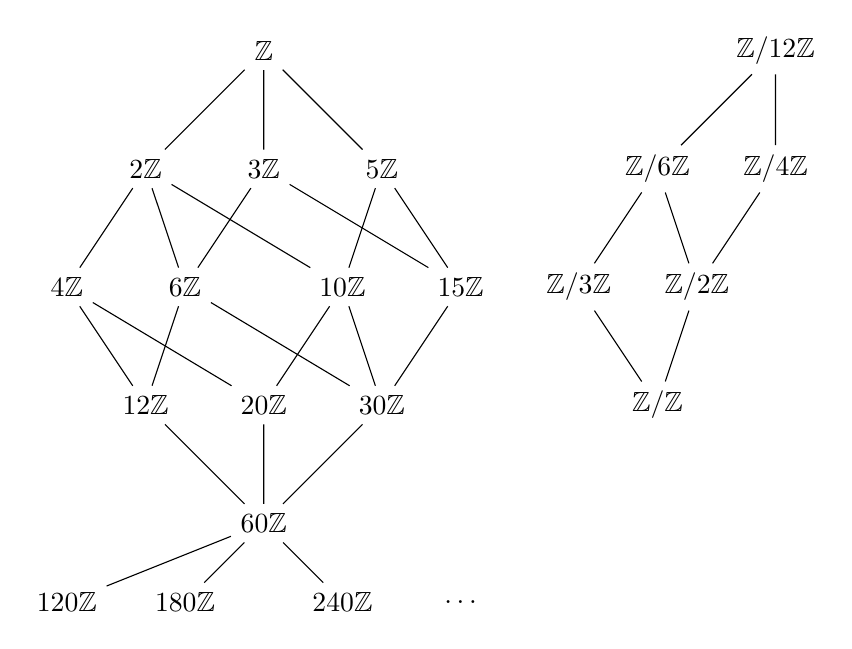
\begin{tikzpicture}[node distance=1.5cm]
\alert<3>{\node (Z) {$\mZ$};

\node (3Z) [below of=Z] {$3\mZ$};
\node (2Z) [left of=3Z] {$2\mZ$};}
\node (5Z) [right of=3Z] {$5\mZ$};

\node (blank) [below of=3Z] {};
\alert<3>{
\node (6Z) [left of=blank,node distance=1cm] {$6\mZ$};
\node (4Z) [left of=6Z] {$4\mZ$};}
\node (10Z) [right of=blank,node distance=1cm] {$10\mZ$};
\node (15Z) [right of=10Z] {$15\mZ$};

\node (20Z) [below of=blank] {$20\mZ$};
\alert<3>{\node (12Z) [left of=20Z] {$12\mZ$};}
\node (30Z) [right of=20Z] {$30\mZ$};

\node (60Z) [below of=20Z] {$60\mZ$};

\node (extraBlank) [below of =60Z, node distance=1cm] {};
\node (180Z) [left of =extraBlank, node distance=1cm] {$180\mZ$};
\node (120Z) [left of =180Z] {$120\mZ$};
\node (240Z) [right of =extraBlank, node distance=1cm] {$240\mZ$};
\node (more) [right of =240Z] {$\ldots$};

\alert<3>{\draw (Z) -- (2Z) -- (4Z) -- (12Z);}
\draw (12Z) -- (60Z);
\alert<3>{\draw (2Z) -- (6Z)-- (12Z);}
\draw (2Z) -- (10Z) -- (20Z) -- (60Z);
\draw (4Z) -- (20Z);
\alert<3>{\draw (Z) -- (3Z) -- (6Z);}
\draw (6Z) -- (30Z) -- (60Z);
\draw (3Z) -- (15Z) -- (30Z);
\draw (Z) -- (5Z) -- (10Z) -- (30Z);
\draw (5Z) -- (15Z);

\draw (60Z) -- (120Z);
\draw (60Z) -- (180Z);
\draw (60Z) -- (240Z);

\onslide<2->{
\node (Z12) [right of =Z, node distance=6.5cm] {$\mZ/12\mZ$};

\node (Z4) [below of =Z12] {$\mZ/4\mZ$};
\node (Z6) [left of =Z4] {$\mZ/6\mZ$};

\node (blank2) [below of =Z4] {};
\node (Z2) [left of =blank2, node distance=1cm] {$\mZ/2\mZ$};
\node (Z3) [left of =Z2] {$\mZ/3\mZ$};

\node (blank3) [below of =blank2] {};
\node (Z1) [left of=blank3] {$\mZ/\mZ$};

\draw (Z12) -- (Z6) -- (Z3) -- (Z1);
\draw (Z6)-- (Z2);
\draw (Z12) -- (Z4) -- (Z2) -- (Z1);
}
\end{tikzpicture}
\end{frame}
\end{document}